\section{Theory: A Toy Graph}\label{sec:theory}

The protocol's prediction is written before any run (Section~\ref{sec:method}). To make it concrete, consider the
smallest graph that contains a correction (Fig.~\ref{fig:toy}). A shared subject $e$ has an old object $D$, asserted
by $n$ passages that each contain $(e, D)$, and a new object $M$, asserted by $k$ passages that each contain $(e, M)$.
Passage edges have weight 1. \emph{Graph A} has passage edges only. \emph{Graph B} adds HippoRAG's count-weighted
relation edges: $e$--$D$ with weight $n$ and $e$--$M$ with weight $k$. The reset vector puts $r_e$ on $e$, $r_D$ on $D$,
$r_M$ on $M$, $r_o$ on each old passage and $r_m$ on each new passage. PPR uses the igraph convention: damping $d$ is the
probability of following an edge, so $\pi = (1-d)\,r + d\,W^\top \pi$ with $W$ the row-normalised weighted adjacency
matrix. Write $x$ for the score of one old passage and $y$ for one new passage.

\begin{proposition}[Shared-subject seed]\label{prop:shared}
With all reset mass on the shared subject ($r_e = 1$),
\begin{align}
\text{Graph A:}\quad x = y &= \frac{d}{(1+d)(n+k)},\\
\text{Graph B:}\quad x = y &= \frac{d}{(2+d)(n+k)}.
\end{align}
\end{proposition}
Seeding only the shared subject therefore never separates old from new passages, whatever $n$ and $k$ are: redundancy
lowers every passage's score equally.

\begin{proposition}[Margin in Graph B]\label{prop:margin}
For a general reset vector,
\begin{equation}
\Delta = x - y = \frac{2(1-d)}{4-d^2}\Big[d\Big(\frac{r_D}{n} - \frac{r_M}{k}\Big) + 2\,(r_o - r_m)\Big],
\label{eq:margin}
\end{equation}
and the coefficient of $r_e$ is $0$.
\end{proposition}
The old passages win ($\Delta > 0$) only through object-specific phrase seeds ($r_D$ versus $r_M$, divided by the number
of passages on each side) and through per-passage seeds ($r_o$ versus $r_m$). Inside the bracket the passage-seed term
has weight $2$ and the phrase term weight $d$, i.e.\ $4\times$ at HippoRAG's $d = 0.5$. For reference, the same derivation for
Graph A gives $\Delta_A = \frac{2(1-d)}{2-d^2}\big[d(r_D/n - r_M/k) + (r_o - r_m)\big]$, again independent of $r_e$.

\begin{corollary}[HippoRAG's seed rule]\label{cor:seed}
HippoRAG divides a phrase's fact score by the number of passages containing the phrase (stage C). If $D$ and $M$ receive
the same fact score $\sigma$ and no passage seeds differ, then $r_D = \sigma/n$, $r_M = \sigma/k$ and
\begin{equation}
\Delta = \frac{2(1-d)}{4-d^2}\; d\,\sigma\Big(\frac{1}{n^2} - \frac{1}{k^2}\Big).
\end{equation}
The side with fewer passages gains per passage: with equal fact scores, a single correction ($k = 1$) against
redundant old support ($n > 1$) has the larger per-passage seed.
\end{corollary}

These are toy-graph results. The real index adds synonym edges, many unrelated facts and passages, min--max
normalisation, top-5 phrase truncation and dense passage seeds for every passage, so the closed forms locate mechanisms
rather than predict magnitudes. Three mechanisms follow: a correction can lose because its object is never seeded
(\emph{seed exclusion}; stages A--C), because old passages crowd the top 5 (\emph{top-5 contamination}; stage E), or
because the seeds that do differ favour the old side (\emph{graph asymmetry}; the bracket in~\eqref{eq:margin}).
All four statements were re-derived symbolically with sympy and checked against igraph's PRPACK solver on the full
(unreduced) toy graph for $n, k \in \{1,2,3,5\}$, $d \in \{0.3, 0.5, 0.85\}$ and 480 random reset vectors (maximum
absolute deviation $2.2\times10^{-16}$; \texttt{experiments/theory/verify\_margin.py}).

\begin{figure}[t]
\centering
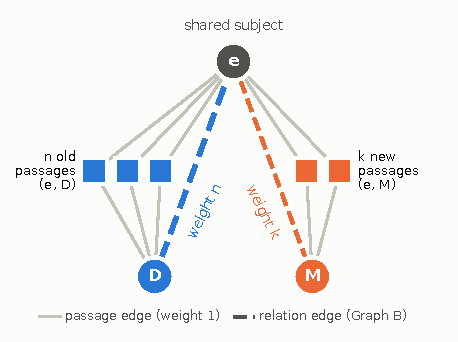
\includegraphics[width=0.82\columnwidth]{figs/toy_graph.pdf}
\caption{The toy graph ($n = 3$, $k = 2$ drawn). Graph A has the passage edges only; Graph B adds the count-weighted
relation edges $e$--$D$ (weight $n$) and $e$--$M$ (weight $k$).}
\label{fig:toy}
\end{figure}
